% !TEX root = base-r.tex

\begin{seeblock}{문자열}{stringr}
  \small\renewcommand{\arraystretch}{1.5}
  \begin{tabular}{c >{\footnotesize} p{0.45\linewidth}}
    \inline{paste(x, y, sep = ' ')} & 여러 개의 벡터 합치기\\
    \inline{paste(x, collapse = ' ')} & 벡터의 원소들 합치기\\
    \inline{grep(pattern, x)} & \inl{x}에서 정규 표현식으로 찾기\\
    \inline{gsub(pattern, replace, x)} & \inl{x}에서 해당하는 항목 대치하기\\
    \inline{toupper(x)} & 대문자화하기\\
    \inline{tolower(x)} & 소문자화하기\\
    \inline{nchar(x)} & 문자열 길이
%    \inl{sprintf(fmt, ...)} & Return a character vector containing a formatted combination of text and variable values.
  \end{tabular}
\end{seeblock}

\begin{block}{팩터}
  \begin{columns}[t]\hfill
    \begin{column}{.45\linewidth}\centering
      \inline{factor(x)}\\벡터를 팩터로 바꾸기. 팩터의 level과 order 설정 가능
    \end{column}
    \begin{column}{.45\linewidth}\centering
      \inline{cut(x, breaks = 4)}\\수로 이루어진 벡터를 잘라서 팩터로 만들기
    \end{column}\hfill
  \end{columns}
\end{block}

{\setbeamercolor{block body}{fg = black, bg = white}
\begin{block}{통계}
  \begin{columns}\hfill\small
    \begin{column}{.45\linewidth}\centering
      
\begin{tikzpicture}[remember picture, overlay]
        \draw[darkgray, dotted, very thick, rounded corners] (-0.45, .25) rectangle (3.35, -2.45);
      \end{tikzpicture}
      \inline{lm(y~x, data=df)}\\선형모형\\[1ex]
      \inline{glm(y~x, data=df)}\\일반화 선형모형\\[1ex]
      \inline{summary}\\모델에서 더 자세한 정보 불러오기.
    \end{column}\hspace{-2ex}
    \begin{column}{.3\linewidth}\centering
      \inline{t.test(x, y)}\\t-검정\\[1ex]
      \inline{pairwise.t.test}\\짝지어진 데이터에 대한 t-검정
    \end{column}\hspace{-2ex}
    \begin{column}{.225\linewidth}\centering
      \inline{prop.test}\\비율검정\\[1ex]
      \inline{aov}\\분산 분석(ANOVA)
    \end{column}\hfill
  \end{columns}
\end{block}

\begin{block}{분포}\small
  \renewcommand{\arraystretch}{1.5}
  \begin{tableau}{| >{\color{black}} c | *{2}{>{\color{black}\centering}m{0.15\linewidth} |} >{\color{black}\centering}m{0.2\linewidth} | >{\color{black}} c |}
    \cline{2-5}
    \multicolumn{1}{l|}{} & 난수 & 확률밀도함수 & 누적분포함수 & 분위수\\\hline
    \rowcolor{secondary} 정규분포 & \inline{rnorm} & \inline{dnorm} & \inline{pnorm} & \inline{qnorm}\\\hline
    푸아송 분포 & \inline{rpois} & \inline{dpois} & \inline{ppois} & \inline{qpois}\\\hline
    \rowcolor{secondary} 이항분포 & \inline{rbinom} & \inline{dbinom} & \inline{pbinom} & \inline{qbinom}\\\hline
    균등분포 & \inline{runif} & \inline{dunif} & \inline{punif} & \inline{qunif}\\\hline
  \end{tableau}
\end{block}
}

\begin{seeblock}{플로팅}{ggplot2}
  \vspace{1ex}
  \begin{columns}\hfill
    \begin{column}{.05\linewidth}\centering
      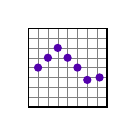
\begin{tikzpicture}[scale = 0.125]
        \fill[white] (0, 0) rectangle (8, 8);
        \draw[step = 1, ultra thin, gray] (0, 0) grid (8, 8);
        
        \foreach \x/\y in {1/4, 2/5, 3/6, 4/5, 5/4, 6/2.75, 7.25/3}
          \fill[violet!65!blue] (\x, \y) circle (12pt);
        \draw (0, 0) rectangle (8, 8);
      \end{tikzpicture}
    \end{column}\hspace{0.1ex}
    \begin{column}{.2\linewidth}\centering
      \inline{plot(x)}\\x의 값(순서대로)
    \end{column}\hspace{-2ex}
    \begin{column}{.05\linewidth}\centering
      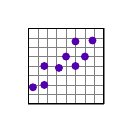
\begin{tikzpicture}[scale = 0.12]
        \fill[white] (0, 0) rectangle (8, 8);
        \draw[step = 1, ultra thin, gray] (0, 0) grid (8, 8);
        
        \foreach \x/\y in {0.5/1.75, 1.7/2, 1.7/4, 3.25/3.8, 4/5, 5/4, 5/6.6, 6/5, 6.8/6.7}
          \fill[violet!65!blue] (\x, \y) circle (12pt);
        \draw (0, 0) rectangle (8, 8);
      \end{tikzpicture}
    \end{column}
    \begin{column}{.25\linewidth}\centering
      \inline{plot(x, y)}\\x에 대한 y의 값
    \end{column}\hspace{-2ex}
    \begin{column}{.05\linewidth}\centering
      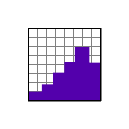
\begin{tikzpicture}[scale = 0.115]
        \fill[white] (0, 0) rectangle (8, 8);
        \draw[step = 1, ultra thin, gray] (0, 0) grid (8, 8);
        
        \fill[violet!65!blue] (0, 0) -- (0, 1) -- (1.5, 1) -- (1.5, 1.8) -- (2.75, 1.8) -- (2.75, 3.1) -- (4, 3.1) -- (4, 4.25) -- (5.15, 4.25) -- (5.15, 5.9) -- (6.75, 5.9) -- (6.75, 4.2) -- (8, 4.2) -- (8, 0) -- cycle;
        
        \draw (0, 0) rectangle (8, 8);
      \end{tikzpicture}
    \end{column}
    \begin{column}{.2\linewidth}\centering
      \inline{hist(x)}\\x의 히스토그램.
    \end{column}\hfill
  \end{columns}
\end{seeblock}

\begin{annotedblock}{날짜}{\textbf{lubridate} 패키지 참조}
\end{annotedblock}
